\documentclass[a4paper, 11pt]{article}

% Locale/encoding with XeTeX: UTF-8 by default, use fontspec
\usepackage{unicode-math}
\usepackage{polyglossia} % Modern replacement for Babel
\setmainlanguage{english}
\usepackage{csquotes} % guillemets
\usepackage{listings}
% Other
\usepackage{fullpage}
\usepackage{graphicx}
%\usepackage{enumerate}
%\usepackage{graphicx}
\lstset{language=Lisp}   
\begin{document}

\title{Final report on the Digital Systems course project}
\author{Nguyễn Lê Thành Dũng \and Thomas Bourgeat}

\maketitle

\section{Summary}

The project's objectives were to design a synchronous circuit usable as a general-purpose processor, and to simulate this processor at the logic gate level using a simulator we wrote ourselves. A clock program running on top of the processor would be used as a demonstration of its capabilities. Those objectives have been met.

Since there's a lot to say here, we will refer you to our two previous intermediate reports for information on the work we did previously.

What follows here is a high-level view of our architecture, combined with a rough description of how we developed the processor. All the details are confined to the appendices.

\section{What's new since last time}

\begin{itemize}
\item In the simulator, we fixed some bugs, and added all the features needed in order to run our processor at a reasonable performance and make the clock demo work. More details in Appendix foobar.
\item In our report on the processor design, we described the kind of architecture we wanted to implement and the rough shape of its machine language. Since then, we have kept the same ideas and filled in the details, following the plans we sketched in that report to their completion.
\end{itemize}

\section{Designing an instruction set}

First, we needed to fix an instruction set that would be expressive enough for our purposes, that is, writing a clock. We concurrently developed, in a single OCaml file, a syntax tree for the S-code (our assembly language), an interpreter for this language, and a program which would count seconds and minutes. 

Our interpreter was meant as a high-level model of how our processor would work in the end. Since  we intended its source code to be amenable to mechanical translation into low-level microcode, we wrote it in an imperative style with global variables. ML-style modules were used to segregate between the memory system and the rest of the program, mirroring the Eval/GC separation in the SCHEME-79 chip.

The \texttt{ocaml/scode.ml} contains the results of this work, including, at the top, the final grammar for the S-code language. As mentioned in the previous report, a S-code program is a tree built up from words and cons cells; the \emph{tag} part of a word specifies the kind of operation to do. The tags can be classified into:
\begin{itemize}
\item Tags to annotate data with their type, e.g. numbers, lists, closures;
\item Opcodes for fundamental operations, e.g. function application, sequencing;
\item Primitive functions, e.g. consing 2 words. We included a lot of special-purpose operations for the project, such as printing a number of seconds to the clock's display
\end{itemize}

\section{From an imperative S-code interpreter to hardware}

The next step was to bridge the gap between a program running on a sophisticated runtime, and the facilities that we could provide with a circuit. On the software side, we converted non-tail function calls into explicit handling of a stack (a global variable), so as to rely only on state transitions (i.e. tail calls) for control. On the hardware side, we needed to implement:
\begin{itemize}
\item The memory system, which previously relied on OCaml's garbage collector.
\item Simple operations on numbers (incrementing and decrementing)
\item And even the mechanism to sequentially execute multiple instructions, which most programmers take for granted!
\end{itemize}
These difficulties are best illustrated by the procedure to retrieve a local variable from a pair of de Bruijn indices: it needs to walk down a linked list, to decrement indices, and to conditionally loop!

Actually, the necessity of executing multiple elementary operations, taking a variable number of cycles, to evaluate a S-code expression led us to take inspiration from CISC processors (indeed, S-code could be considered a very complex instruction set). The technique we used was to consider the S-code instructions as initial states in a state machine encoded as \emph{microcode} and stored in a ROM. Each microinstruction consists of a number of \emph{control signals} which direct the operation of the processor in a single cycle, e.g. by controlling a multiplexer. One can see this process as compiling the relatively high-level S-code to a low-level RISC assembly on the fly.

\section{Overview of the processor}

\subsection{At the hardware level}

The processor's circuit can be divided into multiple functional units, illustrated by figure bloup.
\begin{itemize}
\item The \emph{control unit}, which handles stepping through the microprogram (which is stored in a ROM), maintaining a microprogram counter. It is responsible for conditionals, and issues control signals to the rest of the processor. 
\item The \emph{memory system}, which handles anything memory-related: allocation of cons cells, and dereferencing pointers. It offers a kind of hardware-level abstraction layer: by sending the appropriate opcode, one can allocate a fresh cell without worrying finding an unused memory location. It does \emph{not} do garbage collection (even though we kept the nickname \enquote{GC} from the AI Memos), but is featureful enough to allow our clock to run indefinitely. (See appendix for details.)
\item The \emph{arithmetic logic unit} is a traditional component of any processor. Ours is very minimal, only supporting what we needed for the project. (The original SIMPLE chip (ref biblio) did not even have an ALU, nor did it need one!)
\item The \emph{register array} contains 6 registers, each containing a machine word. Although they are handled uniformly in our implementation, they are meant to be special-purpose: for example, there's a \texttt{Stack} register which holds the control stack (a pointer to a linked list), an \texttt{Expr} register which holds the current expression (analogous to a program counter)\dots There's also a special \texttt{Temp} register, used for allocating conses (for which need \emph{two} words, one from the register array and one from \texttt{Temp}).
\end{itemize}

\subsection{At the microcode level}

The microprogram is a straightforward translation of our OCaml interpreter. Pattern matching on a register's tag is simulated by cutting up the microprogram memory into segments of 32 microinstructions, each of those dedicated to reacting to a single tag, and using a dispatch mechanism to select the starting address corresponding to a tag. We also \enquote{compiled} loops into jumps, for example.

A microinstruction can either:
\begin{itemize}
\item Order around the rest of the circuit, resquesting an elementary operation from the ALU or the GC, or just moving words between registers. The control signals are retrieved from the microinstruction's binary data, without any need for decoding.
\item Jump (contionally or not). 
\item Dispatch on the tag of a register.
\end{itemize}
As can be easily seen, the processor's microcode is akin to a conventional machine language, plus a special dispatch mechanism for S-code interpretation. Indeed, we wrote the microprogram in an assembly-like language with labels (represented as Haskell lists to dispense with the need for a parser), which we then converted to binary with a (micro)assembler.


\section{The clock}

To have a clock running on the processor and displaying the current time on a graphical display, setting up some infrastructure was required both on the simulator side and on the processor side.

Relying on considerable previous experience in writing Tetris clones, we wrote a graphical program using the SDL library for the clock demo. This program, which is integrated with the simulator, shows the time given by the processor on a fake LCD display, responds to user input, and counts the time elapsed since the start of the program (so that it knows when a new second has passed). 

On the processor side, we equip the S-code language with an instruction to wait for the next second, which allows us to write a program counting seconds, minutes and hours in real-time. (See Appendix quux for the program's source in Lisp and in S-code). This instruction triggers outputs from the processor circuit when executed. The simulator reacts to this signal by suspending the simulation, which is then resumed at the next second. 

The display program and the simulation run in two different threads, communicating using shared state.


\section{Auxiliary tools developed for the project}

In addition to the simulator, and the aforementioned graphical program, we developed some software (mostly in Haskell) to help us develop the processor and the clock:
\begin{itemize}
\item The Caillou netlist description language (already mentioned in the previous report)
\item The microassembler, to generate the contents of the microprogram ROM
\item A compiler for a very small Lisp dialect, targeting S-code (since S-code is very close to Lisp, this is a trivial syntactic transformation)
\item A S-code assembler, which linearizes the tree into binary data
\item A little program to debug the microprogram independently from the hardware
\end{itemize}


\newpage
\appendix


\section{Mini-Lisp and S-Code illustrated through the simplest clock program}

\begin{lstlisting}
(defun main ()
  (count-seconds 42))

(defun count-seconds (sec)
  (print-second sec)
  (let ((new-sec (+1 sec)))
    (if (>=60? new-sec)
        ()  
        (synchronize (count-seconds new-sec)))))
\end{lstlisting}

You can see the real program in "./haskell/Lisp/ClockProgram.hs".

\newpage
\section{Functional units in the processor}
\subsection{ALU}
\begin{figure}[h]
\center
\caption{Schematic of the ALU}
   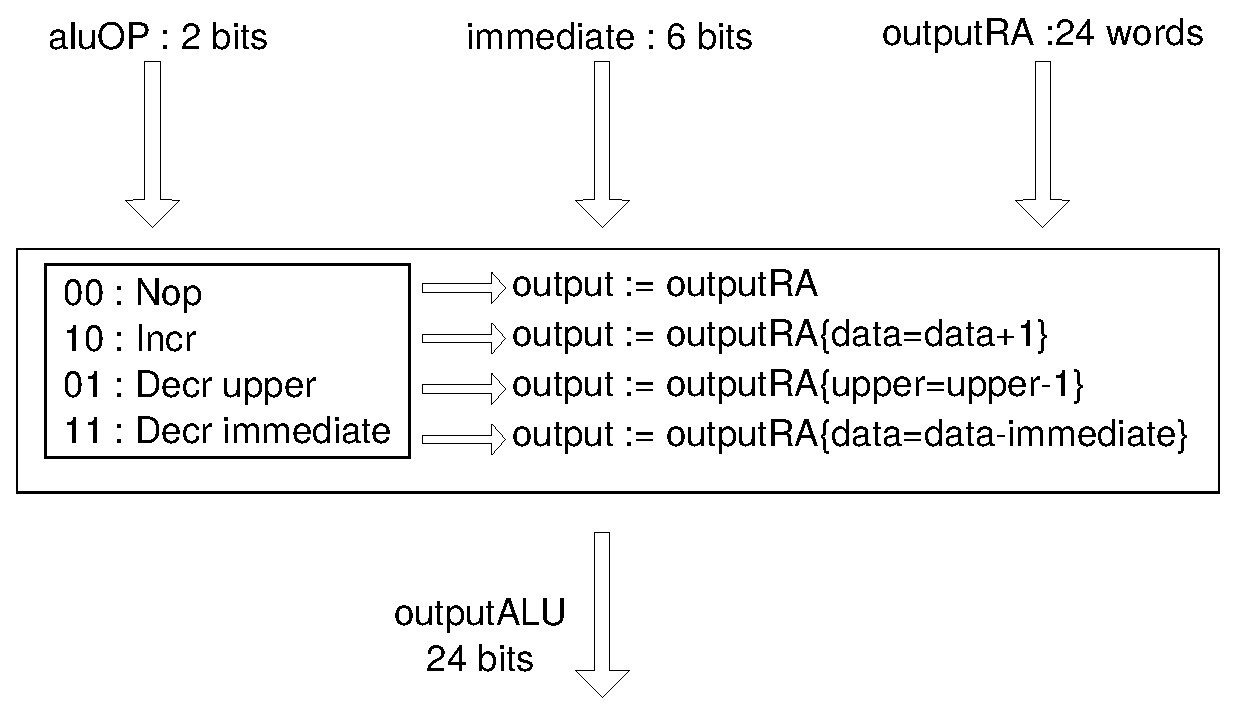
\includegraphics[scale=0.5]{ALU.eps}
\end{figure}

\newpage
\subsection{Memory system}
\begin{figure}[h]
\center
\caption{Schematic of the memory system}
   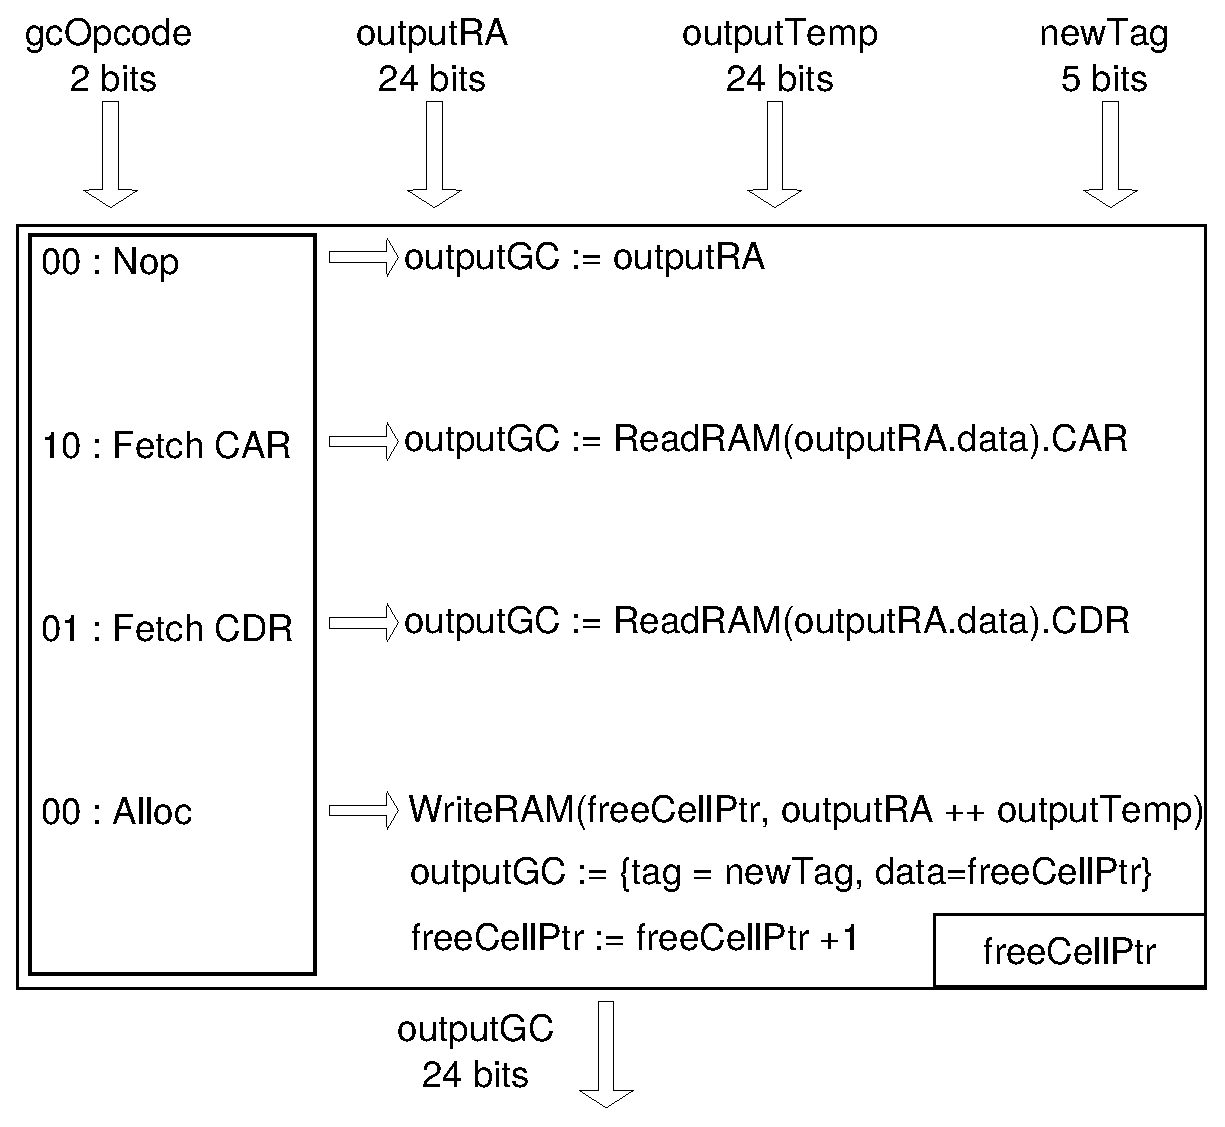
\includegraphics[scale=0.5]{GC.eps}
\end{figure}
\newpage
\subsection{Register Array}
\begin{figure}[h]
\center
\caption{Schematic of the register array}
   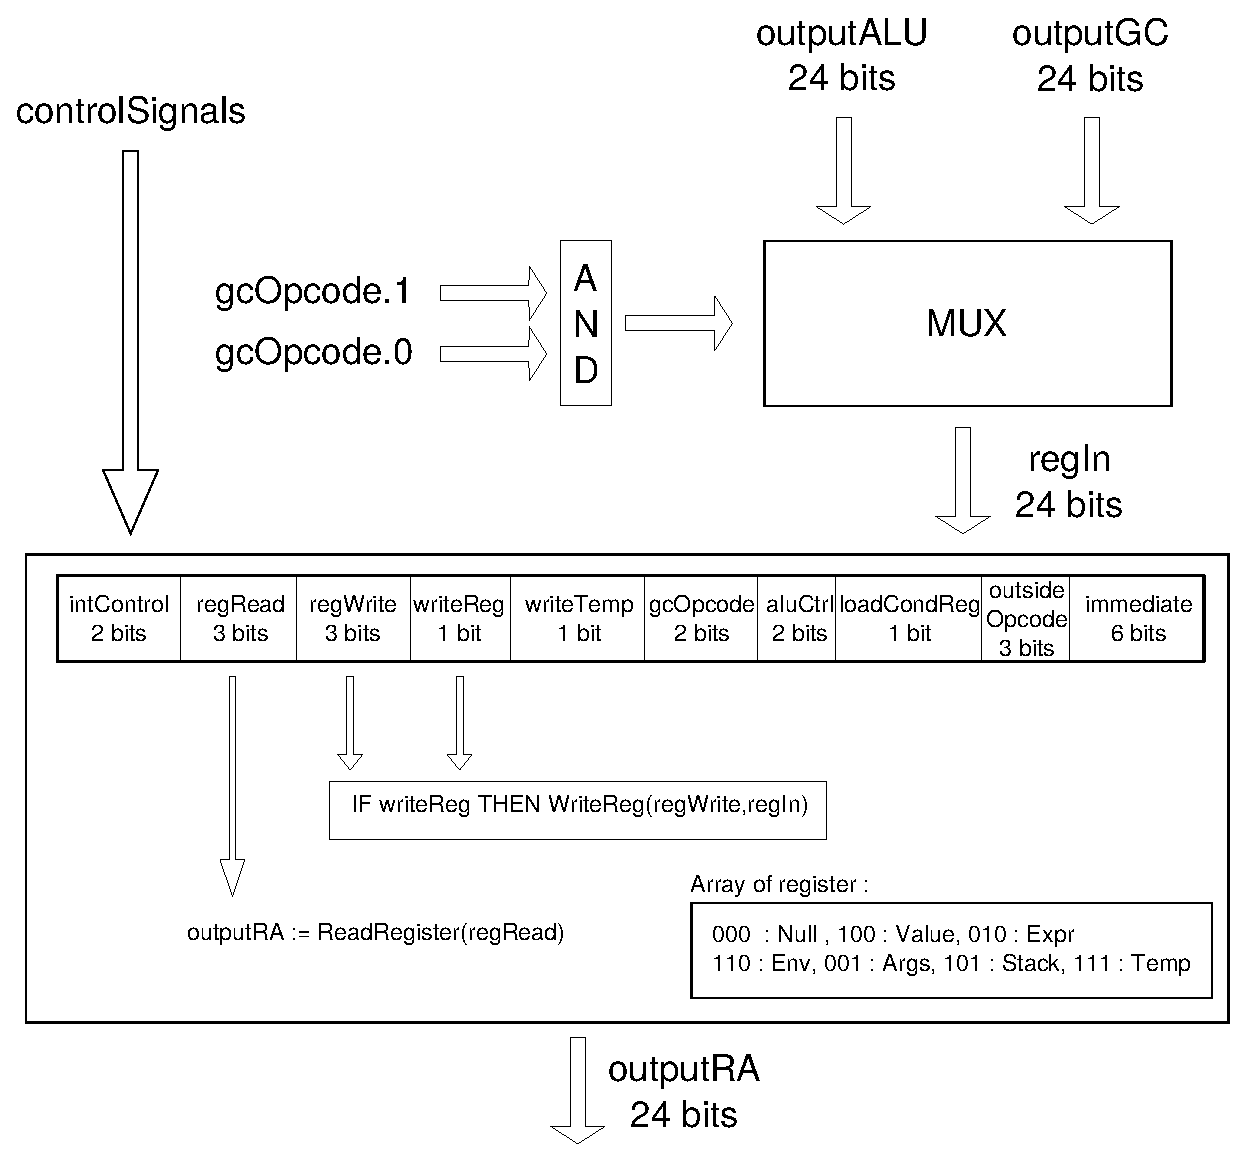
\includegraphics[scale=0.5]{RA.eps}
\end{figure}
\newpage
\subsection{Control unit}
\begin{figure}[h]
\center
\caption{Schematic of the control unit}
   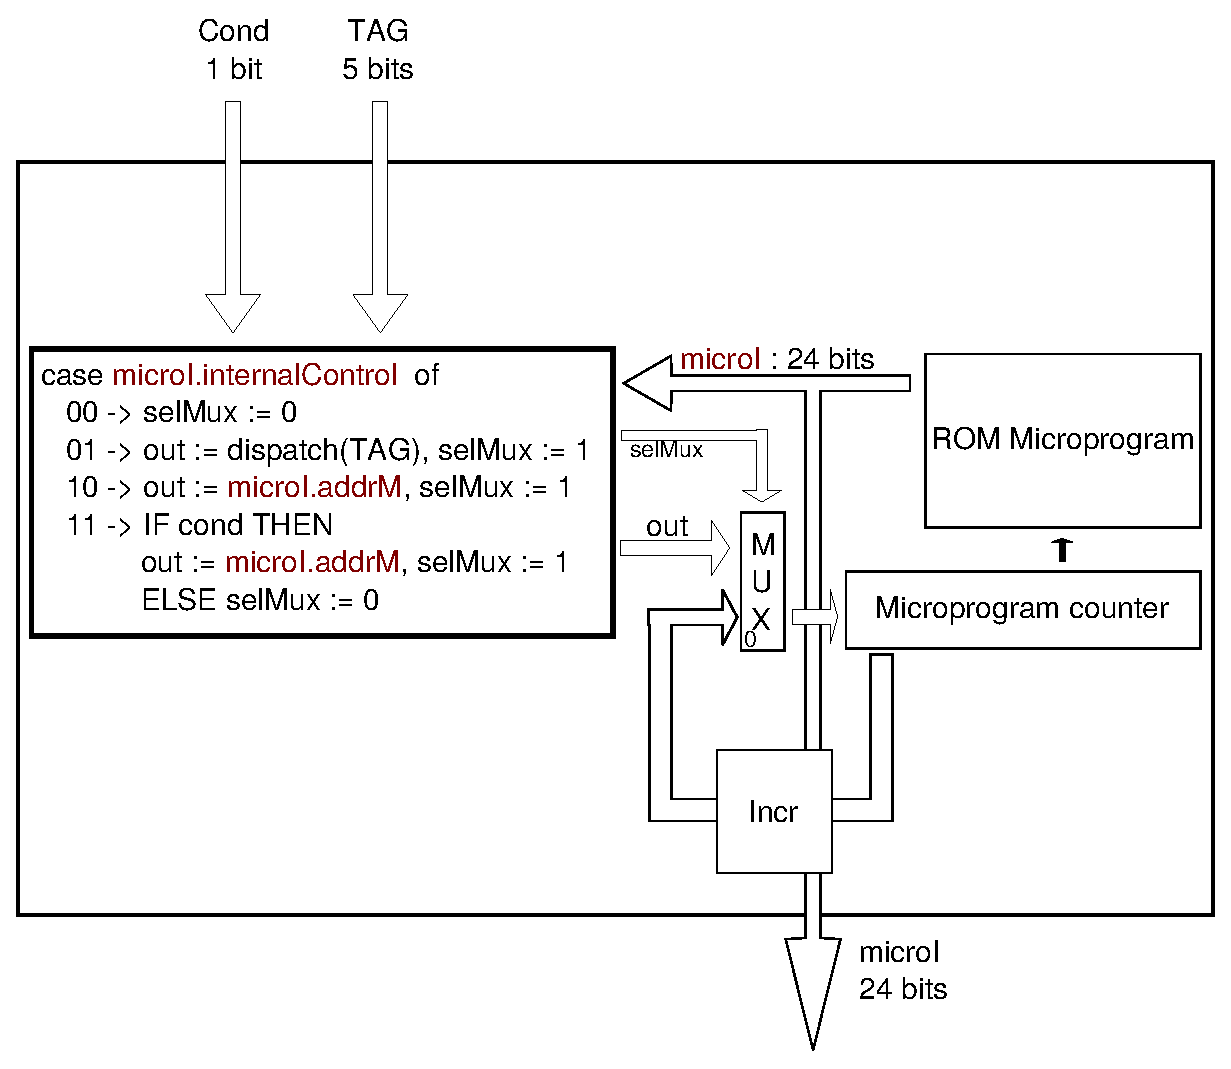
\includegraphics[scale=0.5]{control.eps}
\end{figure}


\section{The microprogram}

\begin{figure}[h]
\center
\caption{Schematic of the microinstruction}
   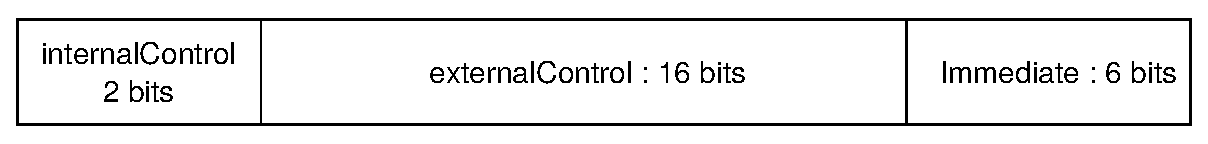
\includegraphics[scale=0.5]{microInstr.eps}
\end{figure}


\section{The Caillou netlist description language}


\section{Source files in the project}
\begin{itemize}
\item "README.md" : Self describing
\item "build.sh" : a script to build the entire project. It generates : rom,
simulator and processor.net. See the README for more precisions.
\end{itemize}
\subsection{./haskell}
\begin{itemize}
\item "generateRom.sh": To generate microprogram and compile the Lisp code.
\item "simulisp.cabal": Configuration file for cabal.
\item ./Caillou:
\begin{itemize}
\item "Arithmetic.hs":  common arithmetical circuits
\item "Circuit.hs": the core interface and typeclasses of Caillou
\item "Examples.hs": some examples of elementary circuits with delays. It was a sandbox.
\item "NetlistGen.hs": Implementation of "Circuit.hs" to generate a Netlist.
\item "Pattern.hs": common combinators for circuits.
\item "Simulation.hs": Implementation of "Circuit.hs" to simulate a circuit.
\end{itemize}
\item ./Lisp : 
\begin{itemize}
\item "AsmScode.hs" : Assembler number 1 from Scode to binary file.
\item "AsmScode2.hs": Assembler number 2 from Scode to binary file. Why? Because
it's not the same algorithm!
\item "ClockProgram.hs"
\end{itemize}
\item ./Processor :
\begin{itemize}
\end{itemize}
\item ./Simulator :
\begin{itemize}
\end{itemize}
\item ./Netlist :
\begin{itemize}
\end{itemize}
\item ./Util :
\begin{itemize}
\end{itemize}
\item ./test :
\begin{itemize}
\end{itemize}
\end{itemize}

\subsection{./ocaml}
\begin{itemize}
\item "scode.ml" : Our software implementation of the processor. 
\end{itemize}
\subsection{./report}
\begin{itemize}
\item Your struly
\end{itemize}


\bibliographystyle{plain}
\bibliography{biblio}

\end{document}
